\documentclass[12pt,fullpage,letterpaper]{article}

\newenvironment{proof}{\noindent{\bf Proof:}}{\qed\bigskip}

\newtheorem{theorem}{Theorem}
\newtheorem{corollary}{Corollary}
\newtheorem{lemma}{Lemma} 
\newtheorem{claim}{Claim}
\newtheorem{fact}{Fact}
\newtheorem{definition}{Definition}
\newtheorem{assumption}{Assumption}
\newtheorem{observation}{Observation}
\newtheorem{example}{Example}
\newcommand{\qed}{\rule{7pt}{7pt}}


\newcommand{\assignment}[4]{
\thispagestyle{plain} 
\newpage
\setcounter{page}{1}
\noindent
\begin{center}
\framebox{ \vbox{ \hbox to 6.28in
{\bf CS6501: Advanced Machine Learning \hfill #1}
\vspace{4mm}
\hbox to 6.28in
{\hspace{2.5in}\large\mbox{Problem Set #2}}
\vspace{4mm}
\hbox to 6.28in
{{\it Handed Out: #3 \hfill Due: #4}}
}}
\end{center}
}

\newcommand{\handout}[3]{
\thispagestyle{plain} 
\newpage
\setcounter{page}{1}
\noindent
\begin{center}
\framebox{ \vbox{ \hbox to 6.28in
{\bf CS6501-01 Advanced Machine Learning  \hfill #1}
\vspace{4mm}
\hbox to 6.28in
{\hspace{2.5in}\large\mbox{#2}}
\vspace{4mm}
\hbox to 6.28in
{{\it Date: #3 \hfill Name (NetID):\makebox[2in]{\hrulefill}}}
}}
\end{center}
}

\newcommand{\solution}[4]{
\thispagestyle{plain} 
\newpage
\setcounter{page}{1}
\noindent
\begin{center}
\framebox{ \vbox{ \hbox to 6.28in
{\bf CS6501 - Advanced Machine Learning \hfill #4}
\vspace{4mm}
\hbox to 6.28in
{\hspace{2.5in}\large\mbox{Problem Set #3}}
\vspace{4mm}
\hbox to 6.28in
{#1 \hfill {\it Handed In: #2}}
}}
\end{center}
\markright{#1}
}

\newenvironment{algorithm}
{\begin{center}
\begin{tabular}{|l|}
\hline
\begin{minipage}{1in}
\begin{tabbing}
\quad\=\qquad\=\qquad\=\qquad\=\qquad\=\qquad\=\qquad\=\kill}
{\end{tabbing}
\end{minipage} \\
\hline
\end{tabular}
\end{center}}

\def\Comment#1{\textsf{\textsl{$\langle\!\langle$#1\/$\rangle\!\rangle$}}}


\usepackage{graphicx}
\usepackage{subfigure}
\usepackage{amsmath}
\usepackage{amssymb}
%\usepackage{qtree}
\usepackage{epsfig}
\usepackage{enumerate}
\usepackage{color}
\usepackage{algorithmic}
\usepackage{hyperref}

%\usepackage{parskip}

\sloppy
\parskip = 0.5cm

\newcommand{\ignore}[1]{}
\newcommand{\pp}{\noindent}
\newcommand{\ov}{\overline}
\newcommand{\bb}[1]{{\bf #1}}
\renewcommand{\labelitemii}{\tiny$\circ$}

\newcommand{\question}[1]{#1}%{}
%\newcommand{\answer}[2]{#1}
%\input{answerdef.tex}
%\newcommand{\answer}[2]{#1}
\newcommand{\answer}[2]{{
\vspace{10pt} 
\color{red}{#2}
\vspace{10pt}
}
}
\newcommand{\comment}[1]{}


\oddsidemargin 0in
\evensidemargin 0in
\textwidth 6.5in
\topmargin -0.5in
\textheight 9.0in

\begin{document}
\setlength{\unitlength}{1mm}

\thispagestyle{plain}
\newpage
\assignment{2017}{2}{Mar 4, 2017}{Mar 15, 2017}

\begin{itemize}
\item Feel free to talk to other members of the class in doing the homework. You should, however,
write down your solution yourself.  Please try to keep the solution brief and clear.

\item Please use Piazza first if you have questions about the homework. Also feel free to come to office hours.

\item Please, no handwritten solutions. You will submit your solution manuscript as a single pdf file. Please use \LaTeX to typeset your solutions.

\item The homework is due at 11:59 PM on the due date. We will be using
Collab for collecting the homework assignments. Please submit your solution manuscript as a pdf file.  Please do NOT hand in a hard copy of your write-up.
Contact the TAs if you are having technical difficulties in 
submitting the assignment. 
\end{itemize}



\section{Training algorithm for Conditional Random Field} 

In this problem set, let's derive an SGD algorithm for CRF. You can refer to the note at \url{http://www.cs.columbia.edu/~mcollins/loglinear.pdf}. However, please write down the answer in your own words.

Recall that in a CRF model, we have input $x$, and a set of possible labels, $y$. We model the conditional probability $P(y\mid x)$ as
\begin{equation}
    P(y\mid x, w) = \frac{\exp(w^T\phi(x,y))}{\sum_{y'} \exp(w^T\phi(x,y')},
\end{equation}
where $w$ is a weight vector and $\phi(x,y)$ is a feature vector.

Given a set of training examples $\{(x_i, y_i)\}_{i=1}^N$, the log-likelihood of the model is $L(w) = \sum_{i=1}^N \log P(y_i\mid x_i, w)$. Then,
the weight vector $w$ can be estimated by the maximum likelihood principle,
\begin{equation}
\label{eq:crf}
    w^* = \arg\max_{w} L(w).
\end{equation}
Recall that to derive the SGD  algorithm for CRF, we first need to rewrite the objective function $L(w)$ in Eq. \eqref{eq:crf} into the form of $\sum_i g_i(w)$.

\begin{itemize}
\item[{\bf Question A}][10points]: Write down the formulation of $g_i(w)$?

\item[ {\bf Question B}][20points]: Write down the gradient of  $g_i(w)$? Please provide complete derivation steps. Hint: The formulation of $\nabla g_i(w)$ is in the lecture slides.



\item[{\bf Question C}][30points]: During the training, we need to evaluate the partition function $\sum_{y'} \exp(w^T\phi(x,y'))$. For an arbitrary output structure, the computational complexity for evaluating the partition function may be exponential in the size of output. However, if the output follows a specific structure, such as a tree or a chain, we can derive a dynamic programming algorithm to compute the partition function.  

Let's assume the CRF model is defined by the following factor graph, and the output structure 
$y=y_1, y_2, y_3, \ldots, y_n$, where each output variable can take a value from 1 to m (i.e., $y_i\in \{1,2,\ldots m\})$.

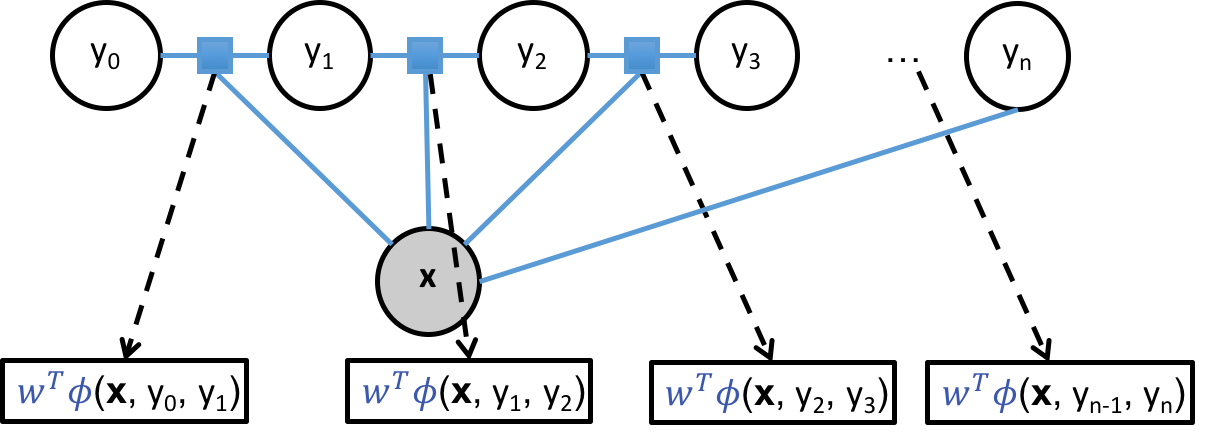
\includegraphics[width=0.8\linewidth]{factor}

That is, $w^T \phi(x,y) = \sum_{i=1}^{n} w^T\phi(x,y_{i-1}, y_i)$.

Design an efficient algorithm for computing $\sum_{y'} \exp(w^T\phi(x,y')) = \sum_{y'} \Pi_{i=1}^{n} \exp(w^T \phi(x, y'_{i-1}, y'_i))$ in $O(nm^2)$ time. Hint: the algorithm is similar to the Viterbi algorithm introduced in Page 32 of \url{http://www.cs.virginia.edu/~kc2wc/teaching/SL17/06-sequence.pdf}.

\end{itemize}
\section{Integer Linear Programming} 
In this problem set, we will derive linear inequalities to represent constraints in integer linear programs. 
Recall the example in page 33 in the slides of Lecture 7. We have three output variables that can take value either $A$ or $B$, and we use binary variable $I_{y_1=A}$ to represent whether the value of $y_1$ is A. Then, the inference problem can be represented as an integer linear programming problem in page 34.  We can use $I_{y_i=A}+I_{y_i=B}=1$ to represent that $y_i$ can either be a A or a B. We can also use $I_{y_1=A}+I_{y_2=A}+I_{y_3=A}  \geq 1$ to represent either $y_1=A$, $y_2 =A$ or  $y_3 =A$.

Note that the constraints in integer linear programming need to be a linear equality or a linear inequality. That is, the constraints are  in a form of $a_1 x_1+ a_2 x_2 + \ldots a_n x_n = b$,  $a_1 x_1+ a_2 x_2 + \ldots a_n x_n \leq b$, or 
$a_1 x_1+ a_2 x_2 + \ldots a_n x_n < b$, where
$x_1, x_2, \ldots, x_n$ are variables and $a_1, a_2, \ldots a_n, b$ are coefficients ($\forall i \quad a_i\in R, b\in R$). Write down a linear  equality or a linear inequality to represent the following constraints.You can use truth table to verify your answers.
\begin{itemize}
\item[{\bf Question A}][5 points]: Write down a linear equality to represent the constraint $y_1=A$.

\item [{\bf Question B}][5 points]:  Write down a linear equality to represent the constraint $y_1 \neq A$ (i.e, $\neg (y_1=A)$).
 
\item [{\bf Question C}][5 points]:  Write down a linear inequality to  represent
the constraint $y_1=A$ and $y_2 =A$ (i.e, $y_1=A\wedge y_2=A$).

\item [{\bf Question D}][5 points]: Write down a linear inequality to represent ``if $y_1=A$ then $y_2 =A$ (i.e., $(y_1=A) \rightarrow (y_2=A)$)''.
Hint: Recall that $x\rightarrow y$ is equivalent to $\neg x \vee y$.  

\item [{\bf Question E}][10 points]:  Write down a linear inequality to represent ``
if $y_{12}=AA$ then $y_1 =A$ and $y_2=A$ (i.e., ($y_{12}=AA) \rightarrow (y_1=A) \wedge (y_2 = A)$)''.
Hint: You can use the property  $x\vee (y \wedge z) \equiv (x\vee y) \wedge (x \vee z)$.

\item [ {\bf Question F}][10 points]: Write down a linear inequality to represent ``
if  $y_1 =A$ and $y_2=A$ then $y_{12}=AA$ (i.e., $(y_1=A) \wedge (y_2 = A) \rightarrow (y_{12}=AA)$)''.
Hint: Use De Morgan's Law  $\neg (x \wedge y) \equiv \neg x \vee \neg y$.
\end{itemize}
\end{document}
